\chapter{Runway design}

	\section{Introduction}
	\paragraph{} The runway is a key piece of the airport and the air side design due to the fact that defines the maximum dimensions of the operative air planes. Its function is to successfully guarantee the landing and takeoff operation.
	
	In order to successfully define the runway, the instructions and requirements given in the Annex 14 given by the ICAO have been followed. 

	\section{Runway Length}
	\paragraph{} The reference field length is defined as the minimum distance needed in order to perform a takeoff operation with the maximum homologated takeoff weight using sea level conditions, without wind and considering 0° slope.  

	In order to calculate the runway length, the first step is to choose the most restrictive air plane that is going to operate on that runway. Afterwards, that length has to be corrected by the runway slope, the altitude of the airport and the mean temperature.

	Due to the fact that the airport has two runways, from now on, the runway used for international flights will be referred as runway 1 and the one used for domestic flights will be named runway 2. 
	
		\subsection{Runway 1}
		The biggest airplanes that will operate on this runway are the Boeing 777-300ER and the Airbus A330-300. 
		
			\subsubsection{Reference Field Length}
			Starting with the B777-300ER, using the ACAP (Aircraft Characteristic for Airport Planning), the values of the MTOW (Maximum TakeOff Weight) and MLW (Maximum Landing Weight) can be obtained. 
			
			\begin{figure}[H]
				\centering
				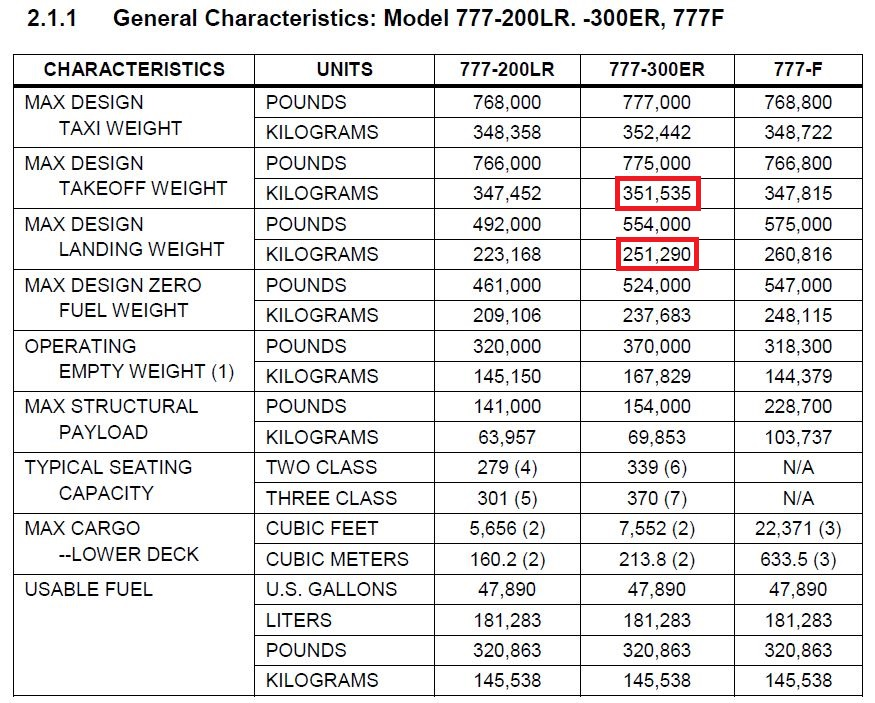
\includegraphics[clip, trim=0cm 0cm 0cm 0cm, width=1\textwidth]{./images/B777/B777MTOW}
				\caption{Maximum weights of the B777 depending on its configuration.} %nom de la figura
				\label{} %per denotar una referencia
			\end{figure}

			The next step is to calculate using the following graph the takeoff distance required with standard day + 15ºC = 30ºC and sea level conditions.
			
			\begin{figure}[H]
				\centering
				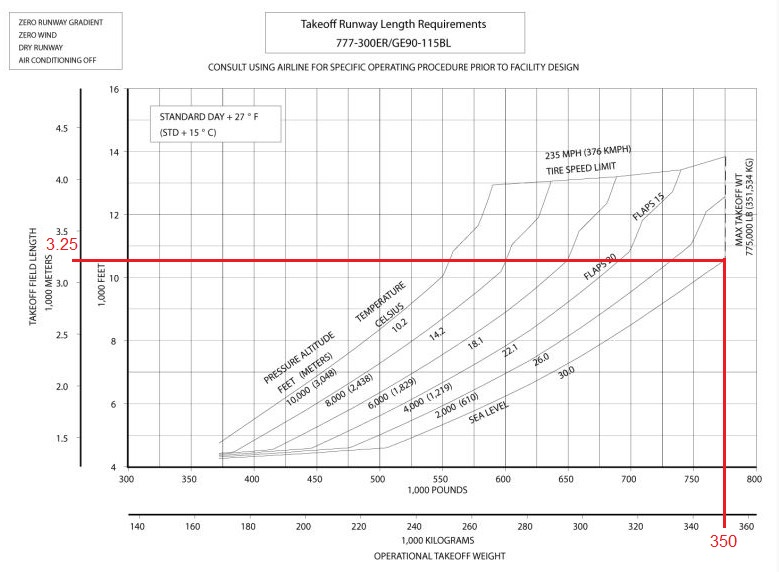
\includegraphics[clip, trim=0cm 0cm 0cm 0cm, width=1\textwidth]{./images/B777/payload-takeoffdistance}
				\caption{Relation between the MTOW and the takeoff distance.} %nom de la figura
				\label{} %per denotar una referencia
			\end{figure}
			
			As it is seen on the graph above, the length taken as reference (LCR) is 3.250m in a standard day+15ºC and sea level conditions. 
			
			The same procedure has to be done with the Airbus A330-300 in order to compare which one is the most restrictive one. Using the ACAP (Aircraft Characteristic for Airport Planning), the MTOW and MLW obtained are the following:
			
			\begin{figure}[H]
				\centering
				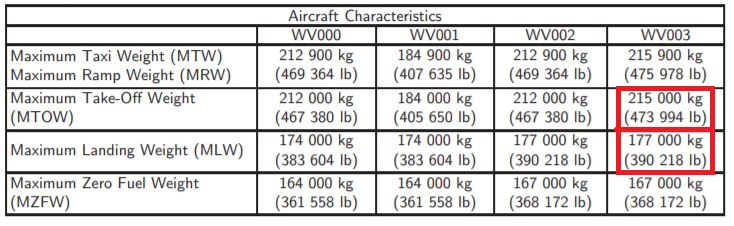
\includegraphics[clip, trim=0cm 0cm 0cm 0cm, width=1\textwidth]{./images/A330/A330}
				\caption{Maximum A330's weights.} %nom de la figura
				\label{} %per denotar una referencia
			\end{figure}
			
			Since the difference on the MTOW and MLW between both planes is greater than a 50\%, the Boeing’s Reference Field Length is chosen as the critical without calculating the Reference Field Length of the A330-300.
			
			Once the most restrictive plane is chosen, the next step is to correct the length following ICAO’s instructions. The equation used to correct the altitude difference is:
			
			\[L_t=RFL*(1+0,07*\frac{\Delta h}{300})\]
			
			Solving the equation for a RFL of 3.250m and an increase on the altitude of 100m, the result obtained is 3326m.
			Since the temperature has already been corrected on the graph and the runway slope is going to be less than 0,5\% and thus, it can be neglected, the final length will be 3.500m rounding up.
		
			\subsubsection{Reference code}
			Using the dimensions of the B777-300ER and the tables given by the ICAO, the number and letter that define the runway can be obtained. 
			
			\begin{figure}[H]
				\centering
				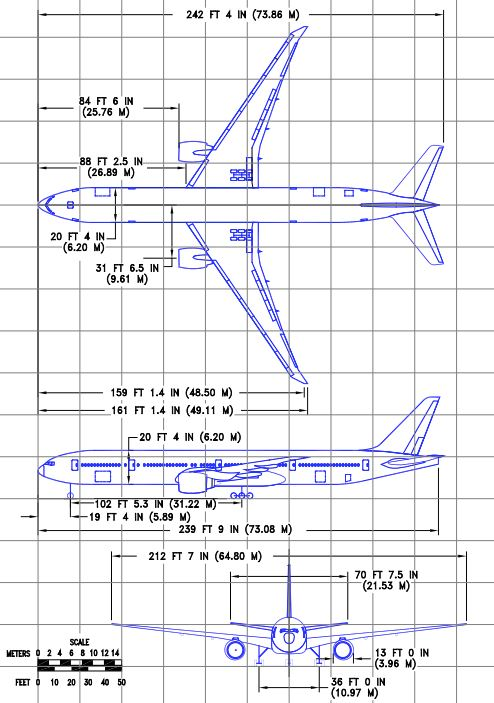
\includegraphics[clip, trim=0cm 0cm 0cm 0cm, width=0.55\textwidth]{./images/B777/Dimensions777}
				\caption{Boeing 777-300ER dimensions.} %nom de la figura
				\label{} %per denotar una referencia
			\end{figure}
				
			\begin{figure}[H]
				\centering
				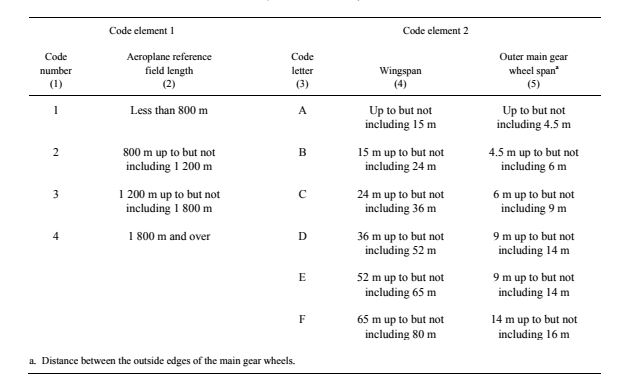
\includegraphics[clip, trim=0cm 0cm 0cm 0cm, width=1\textwidth]{./images/Annex14/Referencecode}
				\caption{Reference code given by the ICAO.} %nom de la figura
				\label{} %per denotar una referencia
			\end{figure}
		
			\paragraph{}Due to the RFL being higher than 1800m , the reference number of the runway is number 4 according to ICAO and due to the dimensions of the air plane B777-300ER, which has a span of 64,8m<65m and a distance between the landing gear of 10,97m<14m, the letter that defines the airport is E.
			
			\subsubsection{Runway width and shoulders}
			\paragraph{}The runway width is obtained using the ICAO recommendations stated on the Annex 14 and the key reference of the runway. 
			
			\begin{figure}[H]
				\centering
				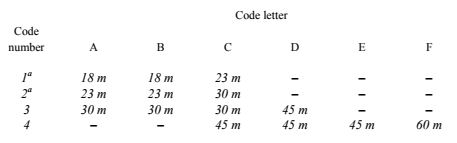
\includegraphics[clip, trim=0cm 0cm 0cm 0cm, width=0.75\textwidth]{./images/Annex14/RunwayWidth}
				\caption{Runway width according to ICAO.} %nom de la figura
				\label{} %per denotar una referencia
			\end{figure}
		
			As it can be seen, and remembering that our key reference is 4E, the minimum runway width needed is 45m. This value has to be further increased with the use of runway shoulders up to a minimum of 60m. 

			\subsubsection{Declared distances}
			\paragraph{} The calculations done in order to obtain the final value can be seen on the airside’s attachments section 1. 
			
			To sum up, the final values obtained are:
			
			\begin{table}[htb]
				\centering
				\begin{tabular}{ll p{5cm}}
					\midrule[2pt]
					Landing Distance Available & 3.500m\\
					TakeOff Distance Available (TODA) & 4.460m\\
					TakeOff Run Available (TORA)& 3.760m \\
					Accelerate-Stop Distance Available (ASDA)& 4.360m\\
					\bottomrule[2pt]
				\end{tabular}
				\caption{Declared distances of  Runway 1}
				\label{DeclareddistancesRW1}
			\end{table}
			
			An schematic figure will be attached in order to ease the understanding of the declared distances:
			
			\begin{figure}[H]
				\centering
				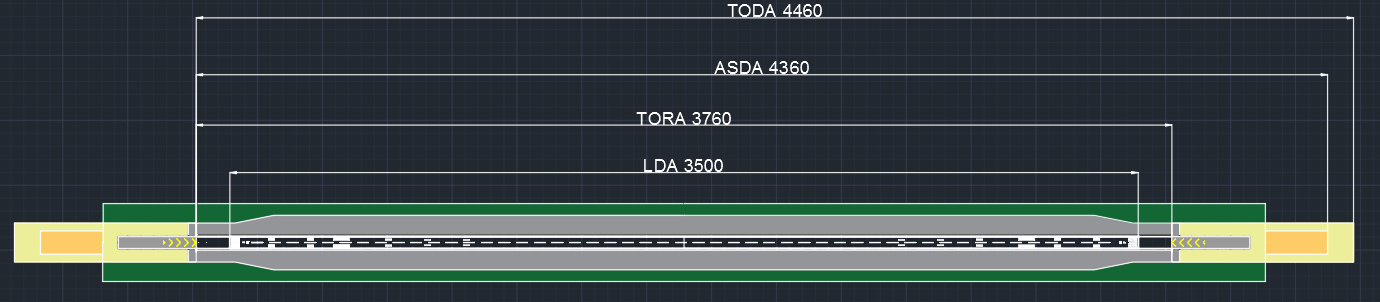
\includegraphics[clip, trim=0cm 0cm 0cm 0cm, width=1\textwidth]{./images/declareddistances/pista}
				\caption{Declared distances on CAD.} %nom de la figura
				\label{} %per denotar una referencia
			\end{figure}
			
			\subsubsection{Runway strips}
			The strip is a delimited area of terrain centred in the runway that has the function of reducing the air plane's risk of getting out of the runway.
			
			According to ICAO's rule number 3.4.2 and 3.4.3, all the runways with a reference number of 4 must contain a strip in each side of the runway's axis. The minimum distance has to be 150m and has to be extended a minimum of 60m after the threshold. 
			Following the rule 3.4.8, the first 150m from the threshold have to be separated at least 75m form the runway's axis. Past those 150m, the strip has to grow linearly until reaching the strip levelled zone.      
			
			\subsubsection{Runway End Safety Areas (RESA)}
			According to ICAO's rule number 3.5.1, the airport with a reference number of 4 has to have a runway end safety area that should extend over a distance of at least 90m. Furthermore, as it is said in the point 3.5.5, the width of a runway end safety area shall be at least twice that of the associated runway. 
			
			\begin{figure}[H]
				\centering
				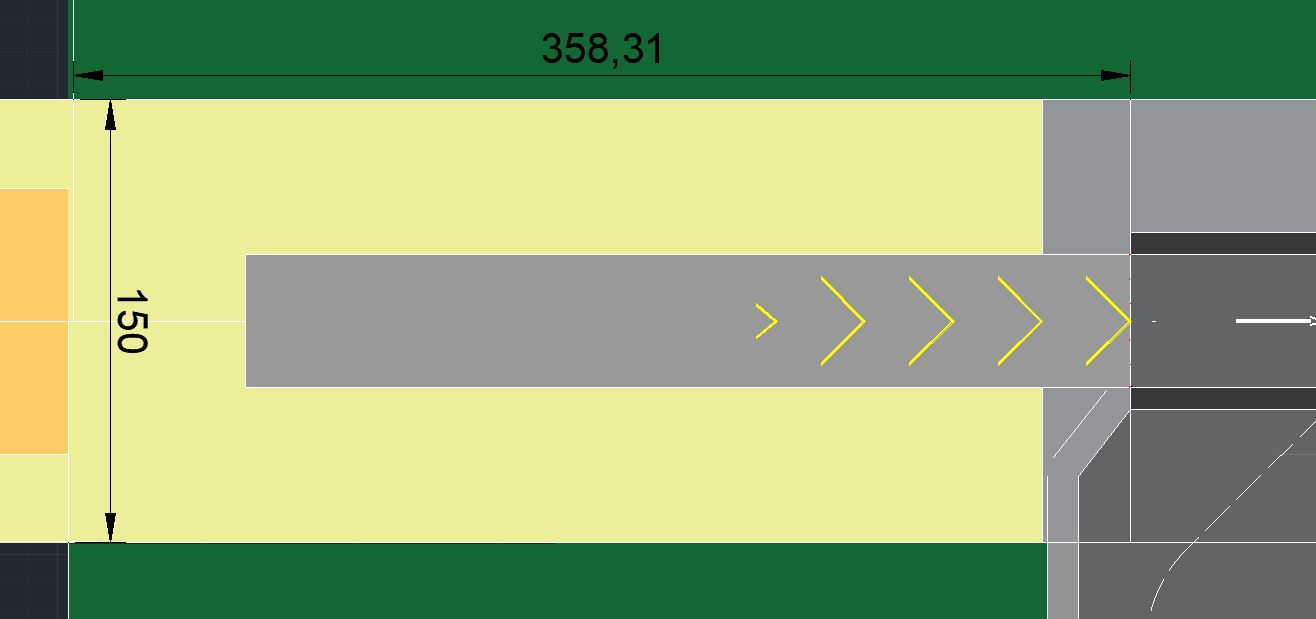
\includegraphics[clip, trim=0cm 0cm 0cm 0cm, width=0.85\textwidth]{./images/declareddistances/RESA}
				\caption{Runway End Safety Area for runway 1.} %nom de la figura
				\label{} %per denotar una referencia
			\end{figure}
		
			As it can be seen, the RESA starts at the end of the strip and its final dimensions are 360m length rounding up and 150m width. 
			
			\subsubsection{Clearway (CWY)}
			Following the recommendation number 3.6.2 and 3.6.3, the Clearway has its beginning at the end of the maximum takeoff distance available and its maximum length should be half that distance.
			
			\begin{figure}[H]
				\centering
				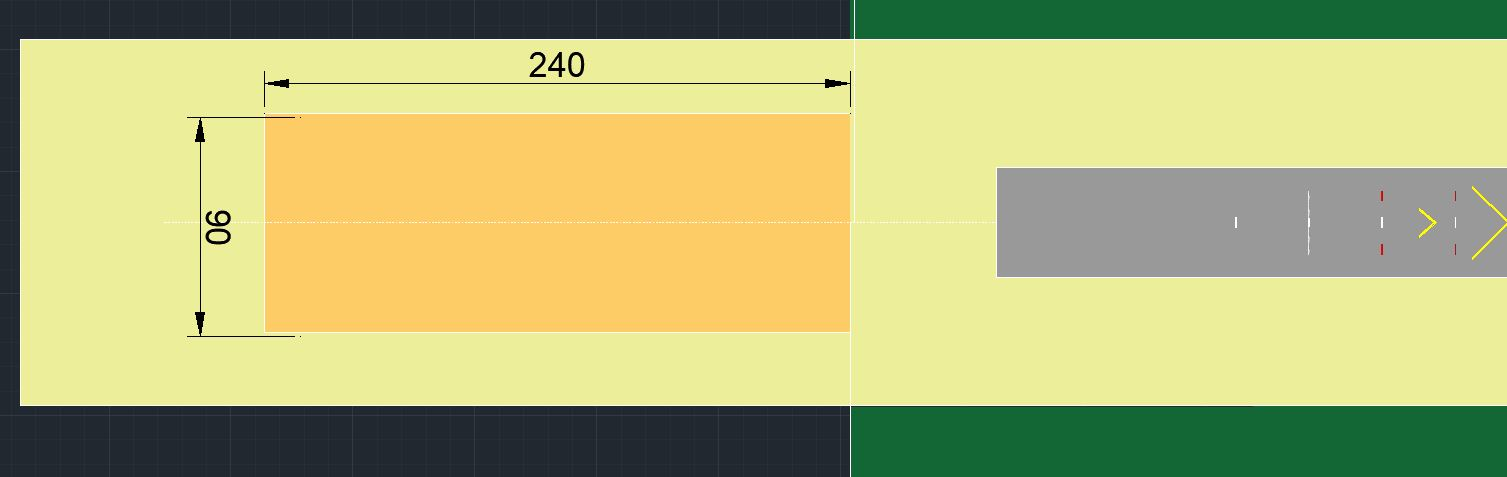
\includegraphics[clip, trim=0cm 0cm 0cm 0cm, width=0.85\textwidth]{./images/declareddistances/CWY}
				\caption{CWY placed at the end of runway 1.} %nom de la figura
				\label{} %per denotar una referencia
			\end{figure}
			
			The final dimensions of the CWY are: 240m length and 90m width. 
			
			\subsubsection{Stopway (SWY)}
			When it comes to the stopway, following the ICAO's rules, the stopway shall have the same width as the runway with which it is associated.

			\begin{figure}[H]
				\centering
				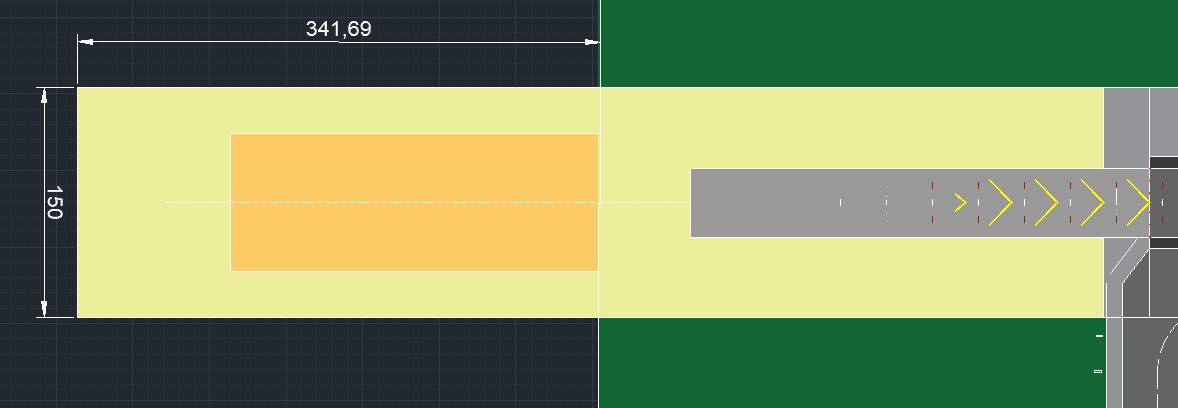
\includegraphics[clip, trim=0cm 0cm 0cm 0cm, width=0.85\textwidth]{./images/declareddistances/SWY}
				\caption{SWY positioning and dimensions.} %nom de la figura
				\label{} %per denotar una referencia
			\end{figure}
		
			As it can be seen, the final values for the SWY are 150m width and 341,69m length.
			
			\subsubsection{Pavement}
			The pavement chosen for the runways will be flexible since it can be easily maintained, it can be restored and there is no risk of fuel leaks during the takeoff and landing performance.
			
			In order to gain a general idea of how the flexible pavement is and how does it work, an image will be attached:
			
			\begin{figure}[H]
				\centering
				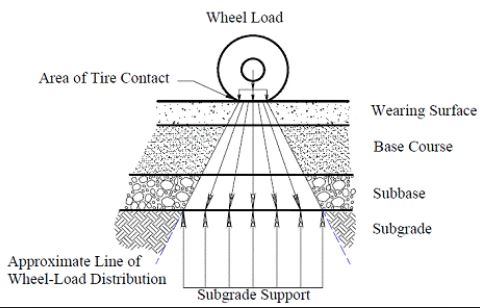
\includegraphics[clip, trim=0cm 0.1cm 0cm 0cm, width=0.75\textwidth]{./images/pavement/flexiblepavement}
				\caption{Flexible pavement layers and load distribution.} %nom de la figura
				\label{} %per denotar una referencia
			\end{figure}
			
			The thickness to be calculated are the wearing surface, the base course and the subbase whilst the subgrade is the natural ground of the area. 
			
			Due to the fact that there is a lot of calculations and graph's interpretation needed in order to calculate the pavement thickness, the explanation step by step will be done in the attachments, chapter 2 section 2. Thus, the only information related to the pavement thickness that will be shown in this section will be the final results obtained and gathered in the following table:
			
			\begin{table}[htb]
				\centering
				\begin{tabular}{ll p{5cm}}
					\midrule[2pt]
					First layer's thickness (\(T_1\))& 14 cm\\
					Second layer's thickness (\(T_2\)) & 25 cm\\
					Third layer's thickness(\(T_3\))& 65,5 cm \\
					Total thickness (\(T_t\))& 104,5 cm\\
					\bottomrule[2pt]
				\end{tabular}
				\caption{Final values of total thickness and each layer's thickness.}
				\label{}
			\end{table}

		\subsection{Runway 2}
		In this case, since this runway is going to be used for domestic flights, the planes that are going to be evaluated are the Boeing 737-800 and the Airbus 320-200.
		\subsubsection{Reference Field Length}
		Searching the values of MTOW and MLW stated on the ACAP of the Boeing 737, the values obtained are 79.000kg for the MTOW and 66.300kg for the MLW.
		
		\begin{figure}[H]
			\centering
			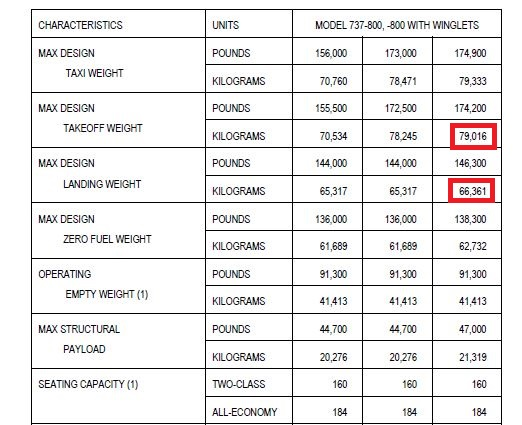
\includegraphics[clip, trim=0cm 0cm 0cm 0cm, width=0.85\textwidth]{./images/B737/B737MTOW}
			\caption{Maximum weights of the B737 depending on its configuration.} %nom de la figura
			\label{} %per denotar una referencia
		\end{figure}
	
		As for the B777, the next step is to calculate using the following graph the takeoff distance required with standard day + 15ºC = 30ºC and sea level conditions using the MTOW.
		
		\begin{figure}[H]
			\centering
			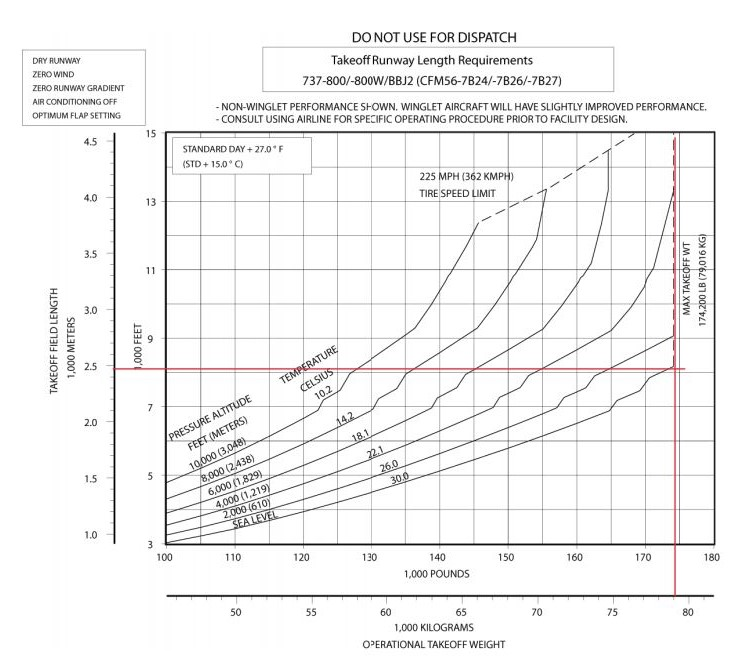
\includegraphics[clip, trim=0cm 0cm 0cm 0cm, width=1\textwidth]{./images/B737/takeoff-weight737}
			\caption{Relation between the MTOW and the takeoff distance.} %nom de la figura
			\label{} %per denotar una referencia
		\end{figure}
	
		The value of the RFL obtained is 2.450m approximately in standard day and sea level conditions. 
		
		The same procedure has to be done with the Airbus A320-200 in order to compare which one is the most restrictive one. Using the ACAP (Aircraft Characteristic for Airport Planning), the MTOW and MLW obtained are the following:
		
		\begin{figure}[H]
			\centering
			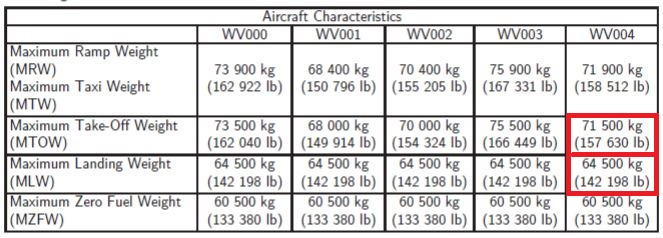
\includegraphics[clip, trim=0cm 0cm 0cm 0cm, width=0.85\textwidth]{./images/A320/A320MTOW}
			\caption{Maximum weights of the A320 depending on its configuration.} %nom de la figura
			\label{} %per denotar una referencia
		\end{figure}
	
		Due to the fact that the MTOW and the MLW of the B737 are higher than the A320 ones, the plane B737 is chosen as the critical for the design of the runway. 		
		
		The next step is to correct the field length using the equation stated above, on the calculations for runway 1. 
	
		\[L_t=RFL*(1+0,07*\frac{\Delta h}{300})\]
		
		Solving the equation for a RFL of 2.450m and an increase on the altitude of 100m, the result obtained is 2500m.
		The same hypotheses used on the runway number 1 will be applied regarding the temperature and slope of the runway.  Thus, the final length will be 2500m.
		
		\subsubsection{Reference code}
		Using the dimensions of the B737-800 and the tables given by the ICAO, the number and letter that define the runway can be obtained. 
		
		\begin{figure}[H]
			\centering
			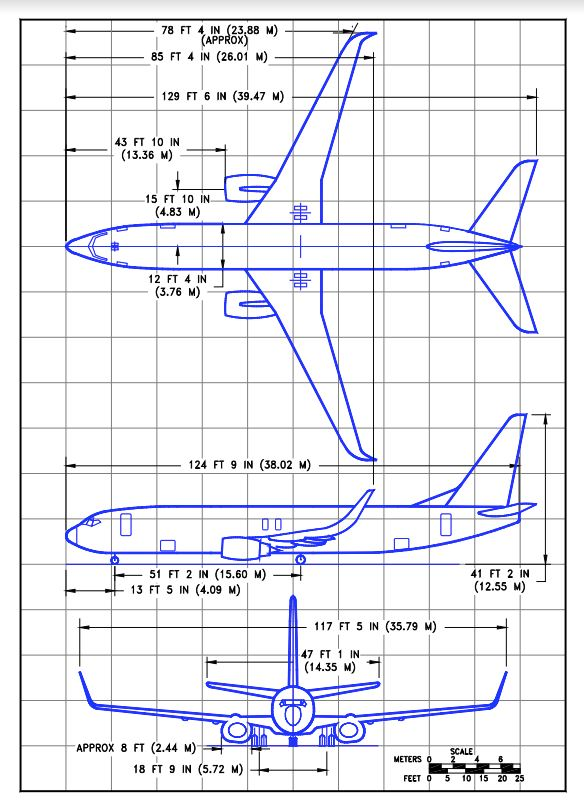
\includegraphics[clip, trim=0cm 0cm 0cm 0cm, width=0.65\textwidth]{./images/B737/737}
			\caption{Boeing 737-800 dimensions.} %nom de la figura
			\label{} %per denotar una referencia
		\end{figure}
	
		\paragraph{}Due to the RFL being higher than 1800m , the reference number of the runway is 4 according to ICAO and due to the dimensions of the air plane B737-800, which has a span of 35,8m<36m and a distance between the landing gear of 6m<9m, the letter that defines the airport is C.
	
		\subsubsection{Runway width and shoulders}
		\paragraph{}The runway width is obtained using the ICAO recommendations stated on the Annex 14 and the key reference of the runway. 
	
		\begin{figure}[H]
			\centering
			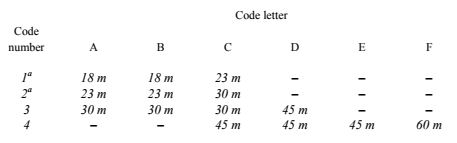
\includegraphics[clip, trim=0cm 0cm 0cm 0cm, width=0.7\textwidth]{./images/Annex14/RunwayWidth}
			\caption{Runway width according to OACI.} %nom de la figura
			\label{} %per denotar una referencia
		\end{figure}
	
		As it can be seen, and remembering that our key reference is 4C, the minimum runway width needed is 45m. This value has to be further increased with the use of runway shoulders up to a minimum of 60m. 
	
		\subsubsection{Declared distances}
		\paragraph{} As for the runway 1, the calculations done in order to obtain the final value can be seen on the airside’s attachments section 1. 
	
		To sum up, the final values obtained are:
	
		\begin{table}[htb]
			\centering
			\begin{tabular}{ll p{5cm}}
				\midrule[2pt]
				Landing Distance Available & 2.500m\\
				TakeOff Distance Available (TODA) & 3.120m\\
				TakeOff Run Available (TORA)& 2.750m\\
				Accelerate-Stop Distance Available (ASDA)& 2.900m\\
				\bottomrule[2pt]
			\end{tabular}
			\caption{Declared distances of  Runway 2}
			\label{DeclareddistancesRW2}
		\end{table}
	
	
		\subsubsection{Runway strips}
		As for the runway 1, due to the fact that both runways share the same reference number and the legislation does not make any distinction using the reference letter, the dimensions of the strips of runway 2 are exactly the same as runway 1. 
		
		\subsubsection{Runway End Saefty Areas (RESA)}
		According to ICAO's rule number 3.5.1, the airport with a 	reference number of 4 has to have a runway end safety area that should extend over a distance of at least 90m. Furthermore, as it is said in the point 3.5.5, the width of a runway end safety area shall be at least twice that of the associated runway. 
	
		\subsubsection{Clearway (CWY)}
		In this case, the clearway dimensions and position is the following:
	
		\begin{figure}[H]
			\centering
			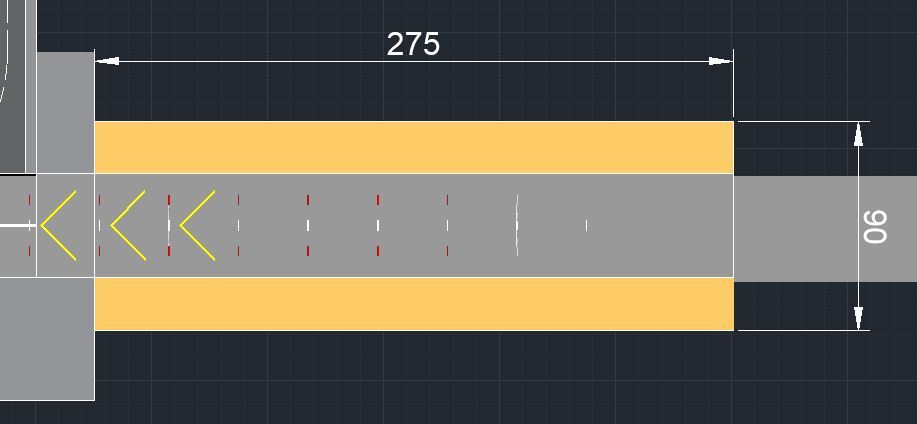
\includegraphics[clip, trim=0cm 0cm 0cm 0cm, width=1\textwidth]{./images/declareddistances/CWY2}
			\caption{CWY placed at the end of runway 2.} %nom de la figura
			\label{} %per denotar una referencia
		\end{figure}
		
		\subsubsection{Pavement}
		The pavement chosen for the runway 2 will be flexible since it can be easily maintained, it can be restored and there is no risk of fuel leaks during the takeoff and landing performance.

		As it was said before, the calculations and graph interpretations for the final runway thickness are further explained in the attachments chapter 2 section 2. Thus, the only information that will be shown in this section will be the final results gathered in the following table:
	
		\begin{table}[htb]
			\centering
			\begin{tabular}{ll p{5cm}}
				\midrule[2pt]
				First layer's thickness (\(T_1\))& 143 cm\\
				Second layer's thickness (\(T_2\)) & 23 cm\\
				Third layer's thickness(\(T_3\))& 55,5 cm \\
				Total thickness (\(T_t\))& 91,5 cm\\
				\bottomrule[2pt]
			\end{tabular}
			\caption{Final values of total thickness and each layer's thickness.}
			\label{}
		\end{table}
		
		